\section{Zielsetzung}
In diesem Versuch soll die Struktur der Elektronenhülle durch ein Elektronenstoßexperiment untersucht werden.
Ziel ist es die Energie zu berechnen, die benötigt wird, um ein Quecksilberatom in den ersten angeregten Zustand zu versetzen. Außerdem soll die
Ionisierungsenergie von Quecksilberatomen berechnet werden. Zusätzlich soll die Energieverteilung der verwendeten Elektronen näher betrachtet werden.

\section{Theorie}
In Abbildung \ref{abb:1} ist der schematische Aufbau dieses Versuches dargestellt. In der evakuierten Röhre befindet sich ein kleiner Tropfen Quecksilber,
ein Teil davon verdampft direkt, bis sich ein Dampfdruckgleichgewicht einstellt. Dieses Dampfdruckleichgewicht und somit auch die Dampfdichte hängt von
der Umgebungstemperatur ab und kann somit variiert werden.
An dem Glühdraht werden durch den Glühelektrischen-Effekt Elektronen emittiert. Zwischen dem Glühdraht der gitterförmigen Beschleunigungselektrode wird eine
Spannung angelegt, die die emittierten Elektronen in Richtung der Beschleunigungselektrode beschleunigt. Die Elektronen haben an der Beschleungigungselektrode
eine Energie von
\begin{equation}
  \label{eq:1}
  \frac{m_0 v_z²}{2} = U_b e_0
\end{equation}
unter der Bedingung, dass die Elektronen keine kinetische Energie besitzen, wenn diese aus dem Glühdraht austreten. Wobei $m_0$ die Masse, $e_0$
die Elementarladung und $v$ die Geschwindigkeit der Elektronen und $U_b$ die Beschleunigungsspannung beschreibt.
Zwischen der Beschleunigungselektrode und der Auffängerelektrode wird eine Gegenspannung $I_A$ angelegt, welche die Elektronen wieder abbremst. Die Elektronen,
die genug Energie haben, um das Bremsfeld zu überwinden, gelangen bis zur Auffängerelektrode und sorgen dann für einen Stromfluss zwischen der Beschleunigungselektrode
und der Auffängerelektrode. Diese Elektronen müssen die folgende Bedingung erfüllen:
\begin{equation}
  \label{eq:2}
  \frac{m_0 v_z²}{2} \geq U_A  e_0
\end{equation}
Die Elektronen die nicht genügend kinetische Energie besitzen, um das Bremsfeld zu überwinden, gelangen zu Beschleunigungselektode zurück.

\begin{figure}
  \centering
  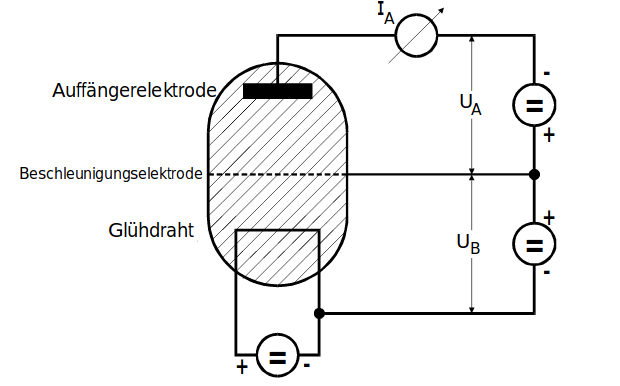
\includegraphics[scale=0.5]{schematischerAufbau.png}
  \caption{Schematischer Aufbau eines Franck-Hertz-Experiments.\cite{Q1}}
  \label{abb:1}
\end{figure}

Da sich in der ganzen Röhre zusätzlich noch Quecksilberatome befinden, kommt es zu zwei verschiedenen Wechselwirkungen zwischen den beschleunigten
Elektronen und den Quecksilberatomen:

Die erste Wechselwirkung ist ein \textbf{elastischer Stoß}. Dieser ist aus energetischer Sicht zu vernachlässigen, da der Energieübertrag sehr gering ist, da die
Masse des Quecksilberatoms sehr viel größer gegenüber der Masse des Elektrons ist. Nicht zu vernachlässigen ist aber die Richtungsänderung, die das Elektron
dadurch erfährt. Denn die oben genannten Gleichungen \eqref{eq:1} und \eqref{eq:2} beziehen sich nur auf die Geschwindigkeiten in z-Richtung.
Wenn ein Elektron also abgelenkt wird und seine Richtung ändert, kann es sein, dass das Elektron nicht mehr genügend Geschwindigkeit in z-Richtung mehr besitzt,
um das Bremsfeld zu überwinden, trotz des geringen Energieübertrags durch den elastischen Stoß.

Die zweite Wechselwirkung ist die \textbf{Anregung der Quecksilberatome}. Diese Wechselwirkung kommt aber nur zustande, wenn das Elektron eine größere Energie
besitzt, als die Energiedifferenz des Grunzustandes und des angeregten Zustandes des Quecksilberatoms. Falls die Bedingung $E \geq E_1-E_0$ erfüllt ist, gibt das
Elektron die Energie $\Delta E = E_1-E_0$ an die Elektronenhülle des Quecksilberatoms ab, welches sich somit im ersten angeregten Zustand befindet.
Kurz darauf emittiert das Quecksilberatom die eben aufgenommene Energie wieder in Form von elektromagnetischer Strahlung mit der Energie
$\Delta E = E_1-E_0 = h \nu$ und fällt in seinen Grundzustand zurück.

Die ideale Franck-Hertz-Kurve ist in Abbildung \ref{abb:2} dargestellt. Hierbei wird der Auffängerstrom $I_A$ gegen die Beschleungigungsspannung $U_B$
aufgetragen. Wenn die Beschleungigunsspannung größer als die Bremsspannung ist, dann steigt der Auffängerstrom $I_A$ immer weiter an. Ist nun aber die
Beschleunigungsspannung so groß, dass die Elektronen die Energie $E_1-E_2$ besitzen, so treten die eben genannten inelastischen Stöße auf mit der Anregung des
Quecksilberatoms. Die Elektronen haben also all ihre Energie an die Quecksilberatome übertragen und können somit die Bremsspannung nicht mehr überwinden. Es
kommt zu dem steilen Abfall des Auffängerstroms.

\begin{figure}
  \centering
  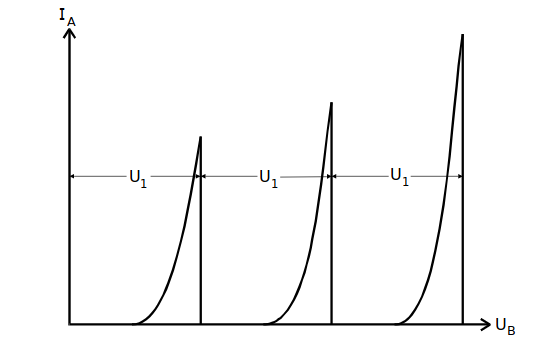
\includegraphics[scale=0.5]{Kurve.png}
  \caption{Idealisierte Franck-Hertz-Kuve.\cite{Q1}}
  \label{abb:2}
\end{figure}

Dies ist dennoch nur eine idealisierte Franck-Hertz-Kurve, es gibt noch einige Einflüsse, die diese verändern:
\begin{itemize}
\item Da der Glühdraht viele Elektronen emittieren soll, wird dieser meist mit einem Oxid eines Erdalkalimetalles überzogen, um die Austrittsarbeit des
Materials zu verringern. Dies führt dazu, dass zwischen dem Glühdraht und der Auffängerelektrode ein \textbf{Kontaktpotential} entsteht (siehe Abbildung \ref{abb:3}),
welches die Franck-Hertz-Kurve um den Wert $K$ verschiebt
\begin{equation}
  K := \frac{1}{e_0}(\Phi_B - \Phi_G)
\end{equation}
\begin{figure}
  \centering
  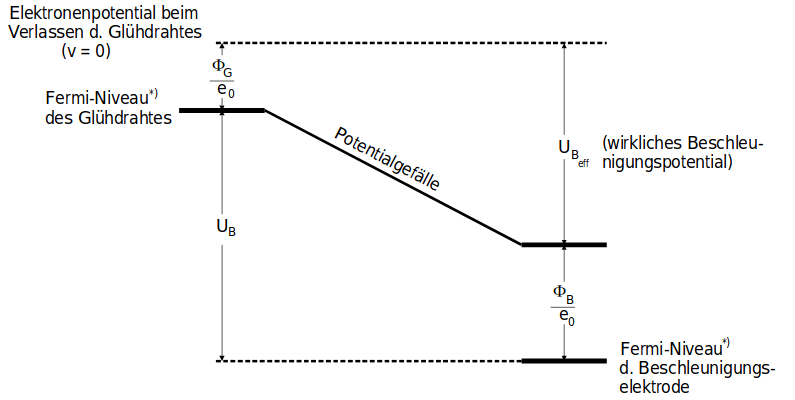
\includegraphics[scale=0.4]{Kontaktpotential.png}
  \caption{Kontaktpotential.\cite{Q1}}
  \label{abb:3}
\end{figure}
\item Bei der idealisierten Franck-Hertz-Kurve wurde bisher davon ausgegangen, dass alle Elektronen die selbe Energie besitzen, dies ist aber nicht der Fall,
da die Elektronen mit unterschiedlichen Anfangsgeschwindigkeiten aus dem Material heraustreten. Dies führt zu einer \textbf{Energieverteilung}, der
Fermi-Dirac-Verteilung. Die Franck-Hertz-Kurve verändert sich dadurch, dass diese bis zum Maximum langsamer ansteigt und nach dem Maximum stetig auf ein
Minimum abfällt und nicht mehr die 0 erreicht.
\item Wie oben schon beschrieben entstehen immer wieder \textbf{elastische Stöße}, hierbei spielt der Energieübertrag kaum eine Rolle, nur die Richtungsänderung
kann man im Bremsbereich nicht vernachlässigen, dies führt zu einer Abflachung und Verbreiterung der Franck-Hertz-Kurve.
\item Derinfluss des Dampfdruckes
Um ein möglichst gute Messung zu erhalten, muss außerdem die mittlere freie Weglänge der Elektronen betrachtet werden, ist diese zu groß wird die
Wahrscheinlichkeit größer, dass die Elektronen ohne jegliche Wechselwirkung mit den Quecksilberatomen bis zu Auffängerelektrode gelangen. Ist die mittlere
freie Weglänge zu klein, dann entstehen mehr elastische Stöße. Es gibt also einen Bereich, in dem die mittlere freie Weglänge optimal ist. Diese kann durch den
\textbf{Sättigungsdampfdruck} $p_{\symup{s}}$ eingestellt werden und dieser ist widerum abhängig von der Umgebungstemperatur
\begin{align*}
  p_{\symup{s}}(T) &= 5,5 \cdot 10⁷ \exp{\left(\frac{-6876}{T}\right)} \\
  \overline{w} &= \frac{0,0029}{p_{\symup{s}}}
\end{align*}
mit $p_{\symup{s}}$ in \si{\milli\bar} und $\overline{w}$ in \si{\centi\meter}.
\end{itemize}

\section{Durchführung}
Der Versuch wird nach Abbildung \ref{abb:4} aufgebaut. Zur Messung der Energieverteilung der Elektronen wird der XY-Schreiber an die Apperatur angeschlossen, wobei
die x-Achse die Bremsspannung $U_A$ und die y-Achse den Auffängerstrom $I_A$ darstellt. Dazu wird die Beschleungigungsspannung $U_b$ konstant auf \SI{11}{\volt} gehalten.
Die Messung wird einmal bei Raumtemperatur $T \approx \SI{23}{\celsius}$ und bei einer Temperatur von $T= \SI{140}{\celsius}-\SI{160}{\celsius}$ durchgeführt. Die Bremsspannung
durchläuft dabei Werte von \SI{0}{\volt} bis \SI{20}{\volt} .Bei diesem Aufbau war darauf zu achten, dass die Heizspannung während der Messung bei etwa \SI{3}{\volt} steht.
Vor der Messung muss außerdem der XY-Schreiber justiert werden. Hierzu wird das Millimeterpapier in den XY-Schreiber eingelegt und zunächst das y-Signal ausgestöpselt.
Daraufhin wird der Nullpunkt an die untere linke Seite des Papiers durch die "zero"-Knöpfe verschoben. Als nächstes wird das y-Signal wieder angebracht um die Empfindlichkeit
der x- und y-Achse einzustellen, hierzu wird die Messung ohne Stift durchlaufen, um die maximale Auslenkung des x- und y-Wertes zu betrachten. Danach werden die
Empfindlichkeiten der Achsen so eingestellt, dass die Messung das ganze Blatt beschreibt. Zuletzt muss die x-Achse noch beschriftet werden, dazu wird die
Bremsspannung immer in \SI{2}{\volt} Schritten eingestellt und mit dem XY-Schreiber ein Punkt gemacht (ohne y-Signal).

Im zweiten Versuchsteil soll die Franck-Hertz-Kurve für verschiedene Temperaturen dargestellt werden. Hierzu werden für 5 verschiedene Messungen Temperaturen im Bereich
\SI{160}{\celsius}-\SI{200}{\celsius} eingestellt. Das x-Signal wird an die Beschleunigungsspannung $U_b$ und das y-Signal an den Auffängerstrom $I_A$ angeschlossen. Die Bremsspannung
$U_A$ beträgt \SI{1}{\volt}, der Messbereich ist $U_b = \SI{0}{\volt}-\SI{60}{\volt}$. Die Justage des XY-Schreibers verläuft wie in dem vorherigen Versuchsteil.

Im letzten Teil soll die Ionisierungsenergie der Quecksilberatome gemessen werden. Bei einer Temperatur von $T= \SI{100}{\celsius}\SI{110}{\celsius}$ wird die Bremsspannung auf
$U_A = \SI{-30}{\volt}$, um mit dem Auffängerstrom nur die positiv geladenen Quecksilberionen zu messen. Auch hier wird an das x-Signal die Beschleunigungsspannung $U_b$ und
an das y-Signal der Auffängerstrom $I_A$ angeschlossen. Der Messbereich ist $U_b = \SI{0}{\volt}-\SI{60}{\volt}$. Auch hier erfolgt die Justage wie in dem ersten Versuchsteil.

\begin{figure}
  \centering
  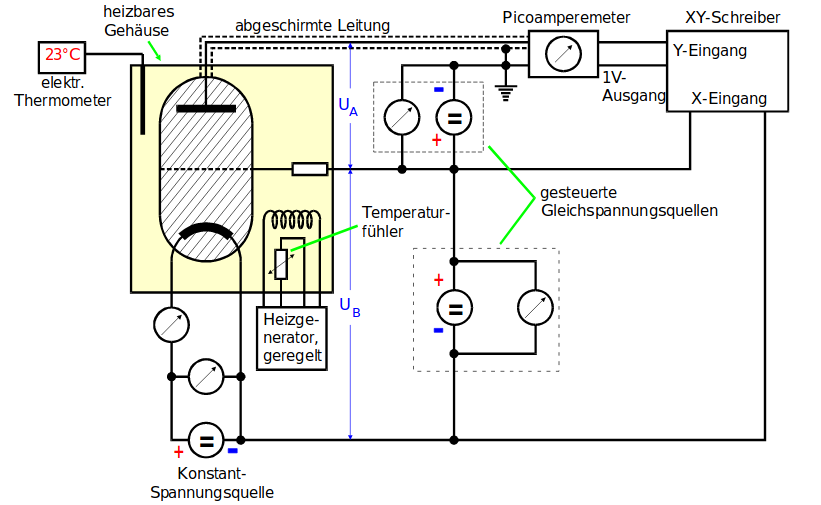
\includegraphics[scale=0.5]{Aufbau.png}
  \caption{Versuchsaufbau.\cite{Q1}}
  \label{abb:4}
\end{figure}
